上一章，我们写了不少 C++ 代码。这一章，一起看看这些代码怎样变成能运行的程序。
先手动走一遍编译过程，再交给 CMake 管理。以后终端刷出一屏报错，你就能先判断卡在哪一步，不用一上来就怀疑人生。

下面的命令都在 Ubuntu 22.04 的 Bash 中运行。每个示例都会写清楚：在哪个目录操作、要建哪些文件、跑完应该看到什么。
打开终端，跟着做就行。

% 保留原有章内一级标题，层级仍由 main.tex 的临时映射控制。
\subsection{C++的编译过程}
\label{sec:build-process}

C++ 从源文件到可执行文件，通常经历以下四步：
\begin{enumerate}
    \item \textbf{预处理（Preprocessing）}：展开头文件、宏和条件编译，得到预处理后的源文件。
    \item \textbf{编译（Compilation）}：检查语法与语义，将预处理结果翻译为汇编代码。
    \item \textbf{汇编（Assembly）}：将汇编代码转换为目标文件（Object File）。
    \item \textbf{链接（Linking）}：把目标文件和所需库组合起来，解析符号引用，生成可执行文件等产物。
\end{enumerate}

\begin{figure}[H]
    \centering
    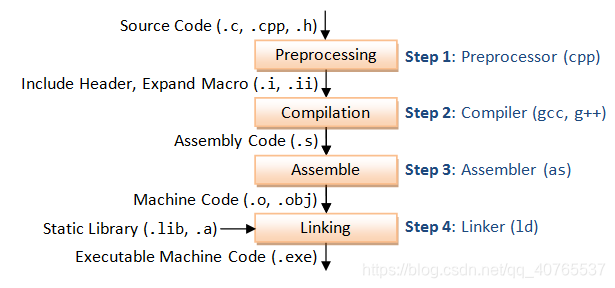
\includegraphics[width=0.7\textwidth]{编译流程.png}
    \caption{C++ 编译过程}
    \label{fig:编译}
\end{figure}

\textbf{预处理：先把这一份源代码准备好}

预处理器先处理那些以 \texttt{\#} 开头的指令。
\texttt{\#include} 引入文件内容，\texttt{\#define} 定义宏，\texttt{\#if} 等指令决定保留哪部分代码。用到宏时，预处理器会按规则展开它。
一个 \texttt{.cpp} 文件，加上它包含的头文件，经过预处理后叫作一个\textbf{翻译单元（Translation Unit）}。
后面编译时，各个翻译单元分别处理。

\begin{note}
同一个头文件，可以在编译不同 \texttt{.cpp} 时分别被处理。
头文件保护（如 \texttt{\#ifndef}/\texttt{\#define}/\texttt{\#endif}）只防止同一翻译单元内重复包含。
写入门工程时，头文件里通常放声明，普通非 \texttt{inline} 函数的定义放在一个 \texttt{.cpp} 里。这样能避免链接时重复定义。
\end{note}

排查问题时，下面这些名字可以帮助定位代码：
\begin{center}
\begin{tabular}{p{0.30\textwidth}p{0.60\textwidth}}
\toprule[1.5pt]
语法 & 作用 \\
\midrule[1pt]
$\_\_FILE\_\_$ & 当前源文件名。\\
$\_\_LINE\_\_$ & 当前源文件行号。\\
$\_\_DATE\_\_$、$\_\_TIME\_\_$ & 源文件被翻译时的日期与时间，不是程序运行时间。\\
$\_\_cplusplus$ & 使用的 C++ 标准版本值；C++17 对应 \texttt{201703L}。\\
$\_\_func\_\_$ & 函数体内可用的标准预定义变量，表示函数名；它不是宏。\\
\bottomrule[1.5pt]
\end{tabular}
\end{center}

\begin{note}
\texttt{\_\_FUNCTION\_\_} 是常见编译器扩展，入门代码优先用 \texttt{\_\_func\_\_}。
\texttt{\_\_STDC\_VERSION\_\_} 表示 C 语言标准版本，不是 C++ 编译器版本；查看 GCC 版本可运行 \texttt{g++ --version}。
\end{note}

\textbf{编译与汇编：检查代码，再生成机器指令}

编译器先分析代码中的词、语法和含义，再生成代码，并按选项进行优化。这些检查分别叫词法、语法和语义分析。
少写分号、调用未声明的函数，通常会在这里报错。

接着，汇编器把汇编代码变成可重定位目标文件（Relocatable Object File）。在 Linux 中，它常以 \texttt{.o} 结尾。
目标文件里有机器代码和数据，还有符号表与重定位信息。你可以先把“符号”理解为函数、变量等的名字。
其中一些符号由本文件定义，另一些还要去其他文件里找。后续链接时，还需要确定相关地址，所以 \texttt{.o} 通常不能直接运行。

\textbf{链接：让调用找到实现}

声明告诉编译器“这个函数怎样调用”，定义给出函数的具体实现。
链接器要把函数调用和对应的实现联系起来，再合并所需代码与数据，处理相关地址。这就是解析符号引用和处理重定位。
如果程序依赖动态库，还会留下一些信息，等加载器处理。

比如，你声明并调用了一个函数，却漏掉了实现所在的目标文件或库。链接器找不到实现，就可能报
\texttt{undefined reference}（未定义引用）。读到这条错误时，先查函数定义有没有参与链接。

\textbf{手动控制四个阶段}

\texttt{g++} 是 GCC 的 C++ 编译驱动程序。通用形式为 $g++\enspace[\text{选项}]\enspace \text{输入文件}\ldots$；不指定停止阶段时，它会继续完成链接。
\begin{center}
\begin{tabular}{p{0.30\textwidth}p{0.60\textwidth}}
\toprule[1.5pt]
参数 & 作用 \\
\midrule[1pt]
$-E$ & 只做预处理。\\
$-S$ & 完成编译后停止，生成汇编文件。\\
$-c$ & 生成目标文件后停止，不链接。\\
$-o\enspace \text{文件}$ & 指定输出文件名。\\
$-std=\text{标准}$ & 选择语言标准，本章使用 \texttt{c++17}。\\
$-I\enspace \text{目录}$ & 增加头文件搜索目录。\\
$-Wall$、$-Wextra$ & 开启常用编译警告。\\
$-g$ & 生成调试信息。\\
\bottomrule[1.5pt]
\end{tabular}
\end{center}
其余参数请查阅 \texttt{man g++} 手册。

\begin{example}[亲眼看到四种产物]
先装好工具，再建一个专门放练习的目录。若你已经用过这个目录名，就换一个，避免覆盖自己的文件。
\begin{tbash}
sudo apt update
sudo apt install build-essential cmake
mkdir -p ~/rm-build-lab/stages
cd ~/rm-build-lab/stages
\end{tbash}
创建 \texttt{hello.cpp}，内容如下：
\begin{tcpp}
#include <iostream>
#define ARMOR_ID 3

int main() {
    std::cout << "armor=" << ARMOR_ID << '\n';
    std::cout << "function=" << __func__ << '\n';
    return 0;
}
\end{tcpp}
留在这个目录里，逐条运行下面的命令。每跑完一步，都看看多了哪个文件：
\begin{tbash}
g++ -std=c++17 -E hello.cpp -o hello.ii
g++ -std=c++17 -S hello.ii -o hello.s
g++ -c hello.s -o hello.o
g++ hello.o -o hello
./hello
\end{tbash}
预期输出两行：\texttt{armor=3} 和 \texttt{function=main}。
再用编辑器打开 \texttt{hello.ii}，搜索 \texttt{armor=}。你会看到这里的 \texttt{ARMOR\_ID} 已经变成了 \texttt{3}。
文件比原来长很多是正常的，头文件内容也被展开进来了。不用从第一页读到最后一页，我们只找刚才那一行。
平时构建时，把这四步交给一条命令就行：
\begin{tbash}
g++ -std=c++17 -Wall -Wextra hello.cpp -o hello
./hello
\end{tbash}
\end{example}

\textbf{静态库与动态库}

有些代码会被多个程序用到，我们可以把它们做成库（Library）。库常见有两种：

\textbf{静态库（Static Library）}通常把多个目标文件打包在一起，Linux 中常见文件名为 \texttt{lib名称.a}。
链接时，链接器把所需目标文件中的代码和数据放进最终产物。

\textbf{动态库或共享库（Shared Library）}在 Linux 中常见文件名为 \texttt{lib名称.so}。
普通动态链接会在构建时记下程序依赖哪些库。程序启动或运行时，再由加载器装入这些库。

\begin{note}
“静态库编译一定更快”和“动态库运行一定更慢”都不是可靠结论。速度取决于具体工程和测量结果。
刚开始先关心一件事：把程序搬到另一台电脑时，还要带上什么？
静态链接某个库后，通常不用再带上这个库的独立文件。动态链接则需要运行环境里有兼容的库。
另外，链接了一个静态库，不代表整个程序都采用了静态链接。性能如何，跑一跑再说，别急着给两种库排战力榜。
\end{note}

\begin{conclusion}
\begin{itemize}
    \item \texttt{.cpp → .ii → .s → .o → 可执行文件} 对应预处理、编译、汇编、链接。
    \item 找不到头文件先查包含路径；语法错误先查源代码；未定义引用先查实现及链接依赖。
    \item 声明用于检查调用，定义提供实现，目标文件承载编译结果，库组织可复用代码。
    \item 静态库与动态库主要影响链接方式和部署条件，不能直接据此判断性能。
\end{itemize}
\end{conclusion}

\begin{exercise}
给装甲板换个编号：把 \texttt{ARMOR\_ID} 改为 \texttt{7}。先直接运行旧的 \texttt{hello}，再重新构建并运行。
两次输出有什么不同？请结合刚才的四步解释原因。
接着故意漏写一个分号，看看哪一步先报错。观察完记得补回来，别给下一节留下伏笔。
\end{exercise}

\subsection{CMake}
\label{sec:cmake-basics}

只有一个源文件时，手写 \texttt{g++} 命令很方便。文件一多，你就得记住：谁依赖谁？哪些文件改过？哪些程序要重新构建？
这些工作可以交给 Make，它按 \texttt{Makefile} 里的规则来做。

\textbf{CMake} 是跨平台的构建系统生成工具。你把工程怎么构建写进 \texttt{CMakeLists.txt}，CMake 再生成 Make、Ninja 或 IDE 使用的构建文件。
之后，相应的构建工具会调用编译器和链接器。
生成器（Generator）决定生成哪种构建文件。CMake 本身不翻译 C++ 代码。

接下来，我们按顺序完成项目配置、添加文件、编译、链接和安装，最后一起读一段实际工程的配置。
先分清三个动作：\textbf{配置与生成}负责读取构建描述、查找依赖、写出构建文件；\textbf{构建}负责真正编译和链接；\textbf{安装}负责按规则复制产物。

看到 \texttt{Configuring done} 和 \texttt{Generating done}，先别开香槟。构建文件准备好了，程序还得接着编译。

\begin{conclusion}
\begin{itemize}
    \item \texttt{CMakeLists.txt} 描述目标和依赖；CMake 读取它并生成构建文件。
    \item Make 或 Ninja 读取生成的规则，安排需要执行的任务。
    \item 编译器和链接器执行这些任务，生成目标文件、库与可执行文件。
    \item 安装按规则复制已有产物；配置成功、构建成功和安装成功是三个不同的检查点。
\end{itemize}
\end{conclusion}

\subsubsection{项目配置}
\label{sec:cmake-config}

先在项目根目录建一个 \texttt{CMakeLists.txt}，文件名的大小写要写对。
里面的命令一般写成 \texttt{命令名(参数...)}。命令名不区分大小写，变量名区分大小写；名称、路径等参数值通常也区分大小写。
开头先写最低 CMake 版本，再用 \texttt{project} 指定语言，让 CMake 检测编译器。

\begin{center}
\begin{tabular}{p{0.49\textwidth}p{0.41\textwidth}}
\toprule[1.5pt]
语法 & 作用 \\
\midrule[1pt]
\texttt{cmake\_minimum\_required(VERSION 版本)} & 声明所需最低版本。\\
\texttt{project(名称 LANGUAGES 语言)} & 设置项目名，启用指定语言。\\
\texttt{set(变量 值...)} & 设置普通变量。\\
\texttt{message(STATUS 内容...)} & 在配置阶段输出信息。\\
\texttt{add\_executable(目标 源文件...)} & 声明一个可执行目标。\\
\texttt{target\_compile\_features(目标 PRIVATE 特性...)} & 为目标指定编译特性，如 C++17。\\
\bottomrule[1.5pt]
\end{tabular}
\end{center}
\texttt{\$\{变量名\}} 表示取变量值，不是 C/C++ 的宏替换。
\texttt{PROJECT\_NAME} 是项目名称，\texttt{CMAKE\_CXX\_COMPILER} 是检测到的 C++ 编译器路径。
\texttt{PRIVATE} 表示这项要求用于当前目标，其他作用域见第~\ref{sec:cmake-scope}~节。

终端命令的通用形式为 $cmake\enspace[\text{选项}]$。构建目录（Build Tree）保存缓存、目标文件和可执行文件，源码目录（Source Tree）保存源代码和构建描述。
\begin{center}
\begin{tabular}{p{0.43\textwidth}p{0.47\textwidth}}
\toprule[1.5pt]
参数 & 作用 \\
\midrule[1pt]
$-S\enspace \text{目录}$ & 指定源码目录。\\
$-B\enspace \text{目录}$ & 指定构建目录，不存在时自动创建。\\
$-D\text{变量}=\text{值}$ & 设置缓存变量，如构建类型。\\
$-G\enspace \text{生成器}$ & 指定生成器，例如 \texttt{Unix Makefiles}。\\
$--build\enspace \text{目录}$ & 调用该构建目录对应的构建工具。\\
$--parallel\enspace \text{数量}$ & 限制并行构建任务数，配合 \texttt{--build} 使用。\\
$--verbose$ & 显示实际构建命令，配合 \texttt{--build} 使用。\\
$--install\enspace \text{目录}$ & 按安装规则复制已构建产物。\\
$--prefix\enspace \text{路径}$ & 指定安装前缀，配合 \texttt{--install} 使用。\\
\bottomrule[1.5pt]
\end{tabular}
\end{center}
其余参数请查阅 \texttt{man cmake}；单条 CMake 语言命令可用 \texttt{cmake --help-command 命令名} 查询。

\begin{example}[先跑通一个最小工程]
在终端新建工程，并复用上节的源文件：
\begin{tbash}
mkdir -p ~/rm-build-lab/hello-cmake
cd ~/rm-build-lab/hello-cmake
cp ../stages/hello.cpp .
\end{tbash}
创建 \texttt{CMakeLists.txt}，完整内容如下。本章采用 CMake 3.16 及以上版本，不需要追求最新版。
\begin{lstlisting}[language=cmake,frame=single,numbers=left]
cmake_minimum_required(VERSION 3.16)
project(hello_cmake LANGUAGES CXX)

set(ARMOR_NAME "training_armor")
message(STATUS "Armor: ${ARMOR_NAME}")
message(STATUS "Compiler: ${CMAKE_CXX_COMPILER}")

add_executable(hello hello.cpp)
target_compile_features(hello PRIVATE cxx_std_17)
\end{lstlisting}
配置、构建和运行：
\begin{tbash}
cmake -S . -B build -DCMAKE_BUILD_TYPE=Debug
cmake --build build --parallel 2
./build/hello
\end{tbash}
配置时应出现 \texttt{Armor: training\_armor} 和编译器路径；运行结果与上节一致。
项目名是 \texttt{hello\_cmake}，目标名是 \texttt{hello}，两者可以不同。
\end{example}

\begin{note}
\texttt{CMakeCache.txt} 会记住编译器、依赖路径等配置。换编译器或生成器时，开一个新的构建目录，别让旧配置继续加戏。
想手动选择 GCC，就在第一次配置时传入 \texttt{-DCMAKE\_CXX\_COMPILER=g++}，不要在 \texttt{project} 后临时修改编译器。
本章使用 Make 等单配置生成器，\texttt{CMAKE\_BUILD\_TYPE=Debug} 用于调试构建；多配置生成器的配置选择用法另查手册。
CUDA 的语言启用与工具链配置见卷二 CUDA 章。
\end{note}

\begin{exercise}
将目标 \texttt{hello} 改名为 \texttt{armor\_hello}，同步修改对应的目标配置，使用新的 \texttt{build-rename} 目录构建并运行。
说明为什么不需要修改 \texttt{project(hello\_cmake ...)}。
\end{exercise}

\subsubsection{添加文件}
\label{sec:cmake-files}

文件准备好后，还得告诉 CMake 怎样使用它们。这里有三件事：列出要编译的源文件、设置头文件搜索目录、查找外部依赖。
CMake 把一个可执行程序或一个库称为目标（Target），后面的配置大多围绕目标来写。
这三件事要分别完成：设置头文件搜索目录不会自动添加源文件，\texttt{find\_package} 也不会替你下载和安装依赖。

\begin{center}
\begin{tabular}{p{0.46\textwidth}p{0.44\textwidth}}
\toprule[1.5pt]
语法 & 作用 \\
\midrule[1pt]
\texttt{set(变量 源文件...)} & 保存显式源文件列表。\\
\texttt{target\_include\_directories(目标 作用域 目录...)} & 为目标设置头文件搜索目录。\\
\texttt{find\_package(包名 REQUIRED)} & 查找已安装的包，缺失时终止配置。\\
\texttt{option(变量 "说明" 默认值)} & 声明可由命令行设置的布尔开关。\\
\texttt{if(条件) ... endif()} & 根据条件执行 CMake 命令。\\
\texttt{target\_compile\_definitions(目标 作用域 宏...)} & 向目标的编译过程传入宏定义。\\
\bottomrule[1.5pt]
\end{tabular}
\end{center}

\begin{example}[为装甲板程序准备三个文件]
\label{ex:armor-sources}
来写一个给装甲板打分的小程序。从这里到安装一节，我们一直用这个 \texttt{armor-demo} 工程，不用每节重新建一套文件。先建目录：
\begin{tbash}
mkdir -p ~/rm-build-lab/armor-demo/include
mkdir -p ~/rm-build-lab/armor-demo/src
cd ~/rm-build-lab/armor-demo
\end{tbash}
创建 \texttt{include/armor.hpp}，只声明接口，并加上头文件保护：
\begin{tcpp}
#ifndef ARMOR_DEMO_ARMOR_HPP
#define ARMOR_DEMO_ARMOR_HPP

int armor_score(int id);

#endif
\end{tcpp}
创建 \texttt{src/armor.cpp}，提供函数定义：
\begin{tcpp}
#include "armor.hpp"

int armor_score(int id) {
    return id * 10;
}
\end{tcpp}
创建 \texttt{src/main.cpp}，使用接口：
\begin{tcpp}
#include "armor.hpp"
#include <iostream>

int main() {
    std::cout << "score=" << armor_score(3) << '\n';
#ifdef SAVE_OUTPUT
    std::cout << "save output enabled\n";
#endif
    return 0;
}
\end{tcpp}
暂时先用上节学过的编译命令验证文件齐全：
\begin{tbash}
g++ -std=c++17 -I include src/main.cpp src/armor.cpp -o armor_manual
./armor_manual
\end{tbash}
预期输出 \texttt{score=30}。其中 \texttt{-I include} 让两个源文件都能找到 \texttt{armor.hpp}。
接下来会为它创建完整的 CMake 构建描述。
\end{example}

头文件通常不用单独编译，但编译器必须找得到它。
你列出要编译的源文件，CMake 据此安排构建。编译器再按包含规则查找头文件，并记录文件之间的依赖，供后续增量构建使用。
所以，源文件列表和头文件路径都要写清楚。

\begin{note}
旧工程可能用 \texttt{file(GLOB\_RECURSE 变量 路径模式)} 递归收集源文件。
我们先把源文件一个个列出来。以后加文件，就顺手改一次列表，检查起来也方便。
用通配符时，要小心把其他程序的 \texttt{main.cpp} 也收进来。两个入口争当主角，链接器可不会帮你选。
\texttt{include\_directories} 设置头文件搜索路径，\texttt{link\_directories} 设置库搜索路径；二者都不等于“把实现链接进程序”。
\end{note}

\begin{exercise}
做两次小型排错练习，每次都从完整命令开始：第一次去掉 \texttt{-I include}，第二次去掉 \texttt{src/armor.cpp}。
分别读一读报错，判断哪次找不到头文件、哪次找不到函数实现。最后恢复完整命令，确认程序能运行。
\end{exercise}

\subsubsection{编译}
\label{sec:cmake-build}

用下面两种形式分别声明可执行目标和库目标：
\begin{quote}
$add\_executable(\text{目标}\enspace \text{源文件}\ldots)$\\
$add\_library(\text{目标}\enspace[\text{类型}]\enspace \text{源文件}\ldots)$
\end{quote}
这两条命令先记下“要构建什么”。等你运行构建命令时，编译器才开始工作。

\begin{center}
\begin{tabular}{p{0.30\textwidth}p{0.60\textwidth}}
\toprule[1.5pt]
参数 & 作用 \\
\midrule[1pt]
目标 & 工程中唯一的逻辑名称，供后续 \texttt{target\_*} 命令引用。\\
源文件 & 要编译的 \texttt{.cpp} 文件，可显式列出或通过变量展开。\\
$STATIC$ & 生成静态库。\\
$SHARED$ & 生成共享库。\\
省略类型 & 根据 \texttt{BUILD\_SHARED\_LIBS} 选择；未设置或为假时默认静态库。\\
\bottomrule[1.5pt]
\end{tabular}
\end{center}

下面还会用到 \texttt{target\_compile\_options}，它为指定目标添加编译选项。
通用形式为：
\begin{quote}
$target\_compile\_options(\text{目标}\enspace \text{作用域}\enspace \text{选项}\ldots)$
\end{quote}
本节用 \texttt{PRIVATE} 把 \texttt{-Wall} 和 \texttt{-Wextra} 仅加给当前目标。
这些选项适用于 GCC、Clang，因此示例先检查编译器标识，再添加它们。
其他选项可查阅编译器手册；这条 CMake 命令的参数可用
\texttt{cmake --help-command target\_compile\_options} 查询。

\begin{example}[一次构建两个源文件]
在示例~\ref{ex:armor-sources}~的 \texttt{armor-demo} 根目录创建 \texttt{CMakeLists.txt}：
\begin{lstlisting}[language=cmake,frame=single,numbers=left]
cmake_minimum_required(VERSION 3.16)
project(armor_demo LANGUAGES CXX)

set(ARMOR_SOURCES src/main.cpp src/armor.cpp)
add_executable(armor_demo ${ARMOR_SOURCES})
target_include_directories(armor_demo PRIVATE
    "${CMAKE_CURRENT_SOURCE_DIR}/include")
target_compile_features(armor_demo PRIVATE cxx_std_17)

if(CMAKE_CXX_COMPILER_ID MATCHES "GNU|Clang")
    target_compile_options(armor_demo PRIVATE -Wall -Wextra)
endif()

option(SAVE_OUTPUT "Enable save-output message" OFF)
if(SAVE_OUTPUT)
    target_compile_definitions(armor_demo PRIVATE SAVE_OUTPUT)
endif()
\end{lstlisting}
\texttt{CMAKE\_CURRENT\_SOURCE\_DIR} 是当前处理的源码目录。
警告选项只加给当前目标；开关只演示条件编译，\textbf{并不真的保存文件}。
\begin{tbash}
cmake -S . -B build -DCMAKE_BUILD_TYPE=Debug
cmake --build build --parallel 2
./build/armor_demo
cmake -S . -B build -DSAVE_OUTPUT=ON
cmake --build build --parallel 2
./build/armor_demo
\end{tbash}
第一次输出 \texttt{score=30}；打开开关并重新构建后，多一行 \texttt{save output enabled}。
\end{example}

\begin{note}
CMake 变量和 C++ 宏处在不同阶段。\texttt{option(SAVE\_OUTPUT ...)} 创建的是配置开关；
\texttt{target\_compile\_definitions} 才把它转换成该目标编译时可见的宏。
\texttt{add\_library(name ...)} 也不保证生成动态库，需要动态库时明确写 \texttt{SHARED}。
\end{note}

\begin{exercise}
给 3 号装甲板开一次“双倍积分”：把 \texttt{armor\_score} 中的乘数改成 \texttt{20}。
只执行构建和运行命令，检查输出是否变成 \texttt{score=60}。
再用 \texttt{-DSAVE\_OUTPUT=OFF} 重新配置并构建，确认提示消失。练完把乘数改回 \texttt{10}，活动结束，积分恢复正常。
\end{exercise}

\subsubsection{链接}
\label{sec:cmake-link}

如果几个程序都要用装甲板打分函数，我们可以把实现做成一个库，让这些程序链接它。
通用形式为：
\begin{quote}
$target\_link\_libraries(\text{目标}\enspace \text{作用域}\enspace \text{依赖}\ldots)$
\end{quote}
第一个参数是已经创建的\textbf{目标名}，不是 \texttt{.o} 文件名。

\begin{center}
\begin{tabular}{p{0.30\textwidth}p{0.60\textwidth}}
\toprule[1.5pt]
参数 & 作用 \\
\midrule[1pt]
目标 & 需要链接依赖的可执行目标或库目标。\\
$PRIVATE$ & 当前目标使用这项依赖；其接口不要求使用者直接使用它。\\
$PUBLIC$ & 当前目标使用依赖，其使用接口也向下游传播。\\
$INTERFACE$ & 仅作为接口要求提供给下游，当前目标不用于自身链接。\\
依赖 & 可为本工程的库目标、包提供的导入目标或库路径等。\\
\bottomrule[1.5pt]
\end{tabular}
\end{center}
链接本工程的库目标时，直接写目标名，CMake 会安排好构建顺序，并找到对应的库文件。
注意 \texttt{armor} 和 \texttt{\$\{armor\}} 的区别：前者是目标名，后者在读取同名变量。如果没设置这个变量，读到的值就可能是空的。

\begin{example}[把实现拆成静态库]
\label{ex:armor-library}
保持三个 C++ 文件不变，将 \texttt{armor-demo/CMakeLists.txt} \textbf{完整替换}为下面内容：
\begin{lstlisting}[language=cmake,frame=single,numbers=left]
cmake_minimum_required(VERSION 3.16)
project(armor_demo LANGUAGES CXX)

add_library(armor STATIC src/armor.cpp)
target_include_directories(armor PUBLIC
    "${CMAKE_CURRENT_SOURCE_DIR}/include")
target_compile_features(armor PUBLIC cxx_std_17)

add_executable(armor_demo src/main.cpp)
target_link_libraries(armor_demo PRIVATE armor)

if(CMAKE_CXX_COMPILER_ID MATCHES "GNU|Clang")
    target_compile_options(armor PRIVATE -Wall -Wextra)
    target_compile_options(armor_demo PRIVATE -Wall -Wextra)
endif()

option(SAVE_OUTPUT "Enable save-output message" OFF)
if(SAVE_OUTPUT)
    target_compile_definitions(armor_demo PRIVATE SAVE_OUTPUT)
endif()
\end{lstlisting}
使用新的构建目录，方便与上一版对照：
\begin{tbash}
cmake -S . -B build-lib -DCMAKE_BUILD_TYPE=Debug
cmake --build build-lib --parallel 2
./build-lib/armor_demo
ls build-lib/libarmor.a
\end{tbash}
预期运行输出 \texttt{score=30}，并能看到静态库 \texttt{libarmor.a}。
\texttt{armor} 把头文件目录设为 \texttt{PUBLIC}，所以链接它的 \texttt{armor\_demo} 也能找到接口头文件。
\end{example}

\begin{conclusion}
\begin{itemize}
    \item \texttt{add\_executable}/\texttt{add\_library} 创建目标；\texttt{target\_*} 为已存在的目标补充要求。
    \item 包含目录解决“头文件在哪”；链接依赖解决“函数实现在哪”；两者各有用途。
    \item 链接一个库目标会带来它公开的使用要求，例如头文件搜索目录。
    \item 静态库的 \texttt{PRIVATE} 依赖仍可能成为最终可执行程序必需的链接项，不能理解成“下游链接命令绝不会出现它”。
\end{itemize}
遇到未定义引用，就沿着这几步查。链接器不接受“我记得写过这个函数”作为证据，得让它真的找到实现。
\end{conclusion}

\begin{exercise}
在 Ubuntu 中把库类型改为 \texttt{SHARED}，用新目录 \texttt{build-shared} 配置、构建并运行，观察生成的 \texttt{libarmor.so}。
记录动态库的文件名，随后将源码中的类型恢复为 \texttt{STATIC}，后续安装示例使用静态库版本。
\end{exercise}

\subsubsection{安装}
\label{sec:cmake-install}

程序已经能在构建目录里运行了。接下来，我们把它放到指定位置，方便以后使用，这一步叫安装（Install）。
按目标声明安装规则的通用形式为：
\begin{quote}
$install(TARGETS\enspace \text{目标}\ldots\enspace[\text{产物类别}\enspace DESTINATION\enspace \text{目录}]\ldots)$
\end{quote}
\begin{center}
\begin{tabular}{p{0.30\textwidth}p{0.60\textwidth}}
\toprule[1.5pt]
参数 & 作用 \\
\midrule[1pt]
$TARGETS$ & 后接已创建的目标名，不写源文件名。\\
$RUNTIME$ & 选择运行时产物；本章用它安装可执行文件。\\
$ARCHIVE$ & 选择归档产物；在本章的 Linux 环境中可用于静态库。\\
$LIBRARY$ & 选择库产物；在本章的 Linux 环境中可用于共享库。\\
$DESTINATION\enspace \text{目录}$ & 指定安装目录；相对目录按安装前缀解析。\\
\bottomrule[1.5pt]
\end{tabular}
\end{center}
本节只安装可执行文件，使用 \texttt{RUNTIME DESTINATION bin}。
安装前缀由终端中的 \texttt{--prefix} 指定；\texttt{bin} 是前缀下的子目录。
其余参数请查阅 \texttt{cmake --help-command install}。

\begin{example}[安装到自己的练习目录]
在示例~\ref{ex:armor-library}~的 \texttt{CMakeLists.txt} 末尾追加：
\begin{lstlisting}[language=cmake,frame=single,numbers=left]
install(TARGETS armor_demo RUNTIME DESTINATION bin)
\end{lstlisting}
在 \texttt{armor-demo} 根目录运行：
\begin{tbash}
cmake -S . -B build-lib -DCMAKE_BUILD_TYPE=Debug
cmake --build build-lib --parallel 2
cmake --install build-lib --prefix "$PWD/stage"
./stage/bin/armor_demo
\end{tbash}
预期出现安装路径 \texttt{stage/bin/armor\_demo}，运行输出 \texttt{score=30}。
该程序已静态链接我们编写的 \texttt{armor} 库，因此这里无需安装独立的 \texttt{libarmor.a}。
\end{example}

\begin{note}
\texttt{cmake --install} 不会自动构建，记得按“配置 → 构建 → 安装”的顺序来。
安装可能覆盖目标位置的同名文件。练习时就用自己的 \texttt{stage} 目录，不需要 \texttt{sudo}，先别急着往系统目录里搬。
如果换成动态库版本，还要带上所需共享库，并设置好运行时搜索路径。只复制一个可执行文件，到了另一台电脑上可能跑不起来。相关细节以后做部署时再展开。
\end{note}

\begin{exercise}
不修改安装规则，将同一程序安装到 \texttt{stage-check} 目录，并从那里运行。
指出安装前缀和 \texttt{DESTINATION bin} 分别对应最终路径的哪一部分。
\end{exercise}

\subsubsection{补充内容}
\label{sec:cmake-scope}

\textbf{目录设置与目标设置}

读旧工程时，你可能会遇到 \texttt{include\_directories}。它会影响当前目录及相关子目录、目标的包含目录设置，不能简单理解成“整个工程都生效”。
我们先用 \texttt{target\_include\_directories} 这类命令：哪个目标需要，就给哪个目标设置。
这里的 \texttt{PRIVATE}、\texttt{PUBLIC}、\texttt{INTERFACE} 决定谁会用到这些配置。名字可能眼熟，但它们和 C++ 类的访问权限是两回事。

\begin{conclusion}
以头文件路径和编译特性为例，三种作用域可这样判断：
\begin{itemize}
    \item \texttt{PRIVATE}：当前目标自己用，例如库内部实现专用的包含目录。
    \item \texttt{PUBLIC}：当前目标和使用它的下游都用，例如示例中的 \texttt{armor.hpp} 所在目录。
    \item \texttt{INTERFACE}：仅下游使用，常见于只提供头文件的接口库。
\end{itemize}
\end{conclusion}

\textbf{把调试函数放进单独的文件}

配置出了问题，又看不出变量里装着什么，就先把它打印出来。
我们把打印操作写成函数，再放进单独的文件，以后就能重复使用。
自定义函数写成 \texttt{function(函数名 参数...) ... endfunction()}。
\texttt{include(模块名)} 用来载入模块，\texttt{list(APPEND 变量 元素...)} 用来往列表中追加元素。
\texttt{CMAKE\_MODULE\_PATH} 是查找自定义模块时使用的目录列表。
把 \texttt{cmake} 目录加入它后，\texttt{include(Function)} 就能找到其中的 \texttt{Function.cmake}。
函数中的 \texttt{if(DEFINED 变量名)} 检查变量是否已定义；已定义但值为空，和根本没定义是两种情况。

\begin{example}[打印编译器与构建类型]
先在 \texttt{armor-demo} 根目录创建模块目录：
\begin{tbash}
mkdir -p cmake
\end{tbash}
新建 \texttt{cmake/Function.cmake}，写入：
\begin{lstlisting}[language=cmake,frame=single,numbers=left]
function(print_var var)
    if(DEFINED ${var})
        message(STATUS "${var} = [${${var}}]")
    else()
        message(STATUS "${var} is not defined")
    endif()
endfunction()
\end{lstlisting}
在 \texttt{CMakeLists.txt} 的 \texttt{project} 后加入：
\begin{lstlisting}[language=cmake,frame=single,numbers=left]
list(APPEND CMAKE_MODULE_PATH
    "${CMAKE_CURRENT_SOURCE_DIR}/cmake")
include(Function)
print_var(CMAKE_CXX_COMPILER)
print_var(CMAKE_BUILD_TYPE)
print_var(NOT_DEFINED_YET)
\end{lstlisting}
运行 \texttt{cmake -S . -B build-lib -DCMAKE\_BUILD\_TYPE=Debug}，预期打印编译器路径、\texttt{Debug} 和未定义变量提示。
\texttt{var} 接收的是变量名。读 \texttt{\$\{\$\{var\}\}} 时，从里往外看：先拿到名字，再读取这个名字对应的值。
空字符串也可以直接输出，不用特意截取最后一个字符或补换行。
\end{example}

\begin{figure}[H]
    \centering
    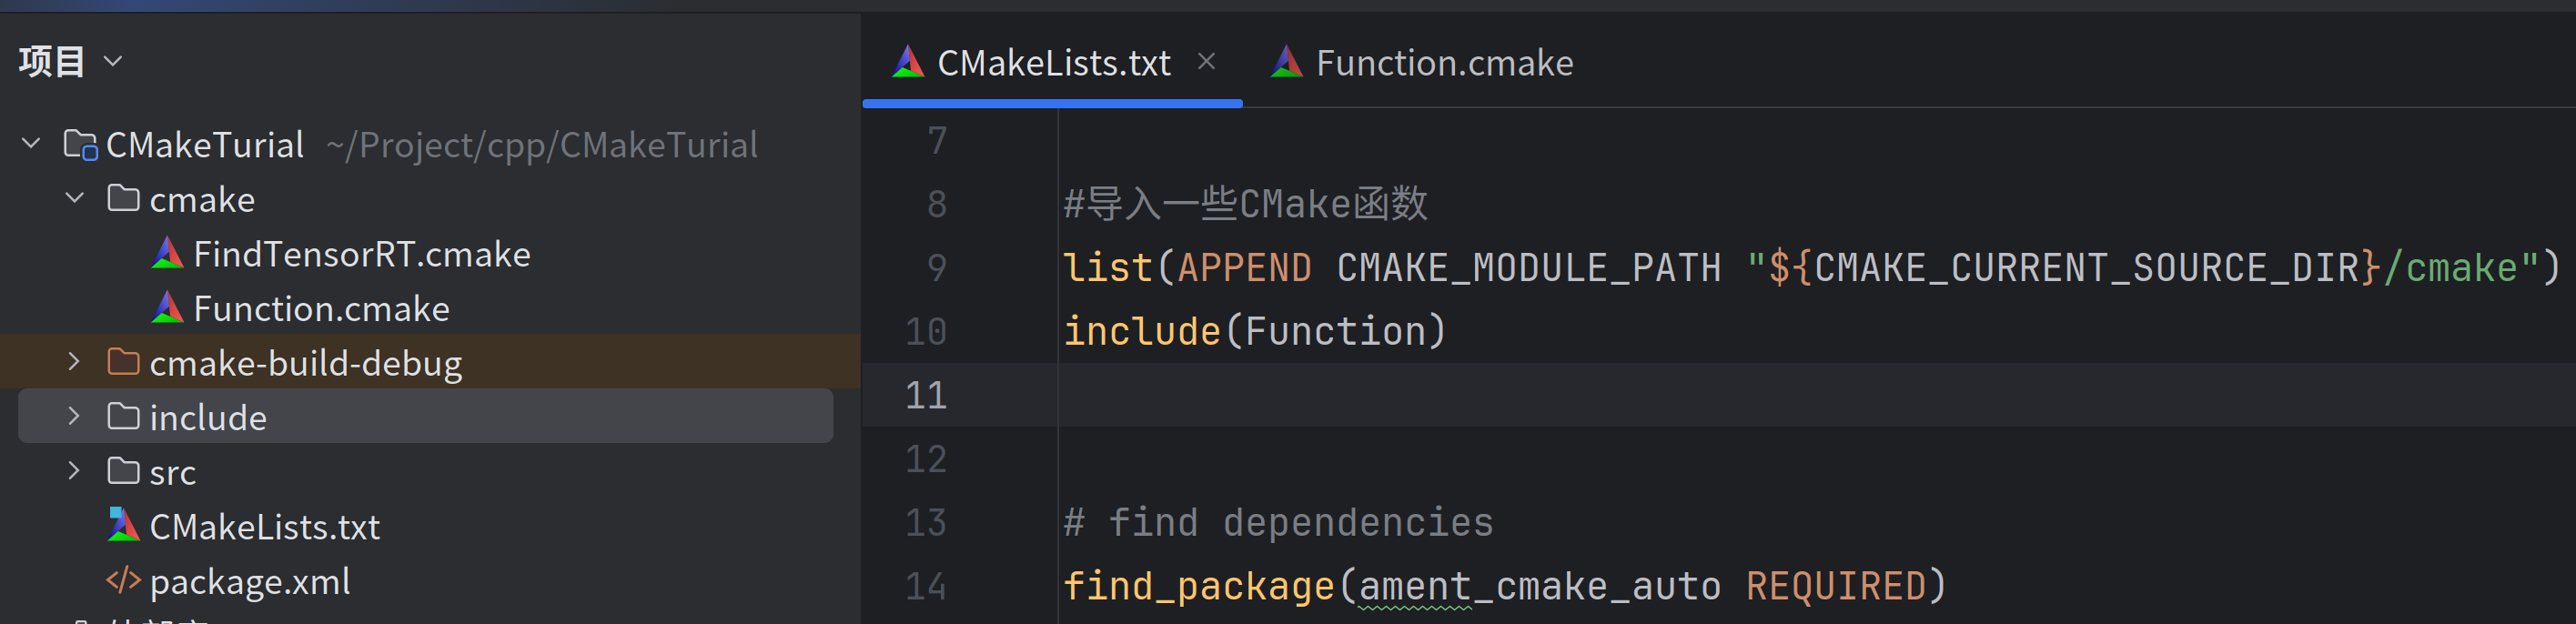
\includegraphics[width=0.7\textwidth]{cmake函数.png}
    \caption{原工程中拆分 CMake 函数文件的结构示意；练习以正文给出的文件路径为准}
    \label{fig:cmakeFunction}
\end{figure}

\textbf{按失败阶段排查}

先别和满屏红字对线，我们从第一处错误看起。
后面的“构建失败”往往只是前面出错后的结果。先判断它发生在哪个阶段，再按下面的方向查，通常比盲目改配置省事。
\begin{center}
\begin{tabular}{p{0.39\textwidth}p{0.51\textwidth}}
\toprule[1.5pt]
命令 / 现象 & 作用 / 排查方向 \\
\midrule[1pt]
配置时报找不到包 & 检查开发包是否安装，以及包配置文件路径。\\
\texttt{No such file or directory}（头文件） & 检查文件名与目标的包含目录。\\
\texttt{undefined reference} & 检查函数定义、签名，以及源文件或库是否参与链接。\\
\texttt{multiple definition} & 检查普通函数是否被重复定义或重复加入目标。\\
\texttt{error while loading shared libraries} & 程序已构建，但运行时找不到所需共享库。\\
\texttt{cmake --build build-lib --verbose} & 查看实际编译与链接命令；无改动时可能没有命令可显示。\\
\bottomrule[1.5pt]
\end{tabular}
\end{center}

\begin{exercise}
在静态库示例中把 \texttt{armor} 的包含目录作用域从 \texttt{PUBLIC} 改为 \texttt{PRIVATE}，重新构建。
指出失败的是库还是可执行目标，解释原因并恢复原配置。
\end{exercise}

\subsubsection{实例}
\label{sec:cmake-opencv}

\textbf{使用外部依赖：OpenCV 图像读取}

自己的库已经能用了，再试试别人写好的 OpenCV。
步骤还是刚才那几步：查找依赖、创建目标、设置包含目录、链接依赖。
\texttt{find\_package(OpenCV REQUIRED)} 查找 OpenCV 提供的包信息；
\texttt{OpenCV\_INCLUDE\_DIRS} 是包含目录，\texttt{OpenCV\_LIBS} 是需要链接的库列表。

\begin{example}[从零编译并显示图像]
在 Ubuntu 桌面环境中安装开发包，建立独立目录：
\begin{tbash}
sudo apt install libopencv-dev
mkdir -p ~/rm-build-lab/opencv-demo
cd ~/rm-build-lab/opencv-demo
\end{tbash}
创建 \texttt{main.cpp}：
\begin{tcpp}
#include <opencv2/opencv.hpp>
#include <iostream>

int main(int argc, char** argv) {
    if (argc != 2) {
        std::cerr << "Usage: image_viewer <image_path>\n";
        return 1;
    }
    const cv::Mat image = cv::imread(argv[1]);
    if (image.empty()) {
        std::cerr << "Cannot read image: " << argv[1] << '\n';
        return 2;
    }
    std::cout << "size=" << image.cols << 'x' << image.rows << '\n';
    cv::imshow("Armor image", image);
    cv::waitKey(0);
    return 0;
}
\end{tcpp}
创建 \texttt{CMakeLists.txt}：
\begin{lstlisting}[language=cmake,frame=single,numbers=left]
cmake_minimum_required(VERSION 3.16)
project(opencv_demo LANGUAGES CXX)

find_package(OpenCV REQUIRED)
add_executable(image_viewer main.cpp)
target_compile_features(image_viewer PRIVATE cxx_std_17)
target_include_directories(image_viewer PRIVATE ${OpenCV_INCLUDE_DIRS})
target_link_libraries(image_viewer PRIVATE ${OpenCV_LIBS})
\end{lstlisting}
先生成一张纯文本格式的测试图，不需要额外下载素材：
\begin{tbash}
printf 'P3\n2 2\n255\n255 0 0  0 255 0\n0 0 255  255 255 255\n' > test.ppm
cmake -S . -B build -DCMAKE_BUILD_TYPE=Debug
cmake --build build --parallel 2
./build/image_viewer test.ppm
\end{tbash}
运行后应输出 \texttt{size=2x2}，并打开显示测试图的窗口。在图像窗口中按任意键，程序就会结束。
这张图只有四个像素，先委屈一下你的显卡。跑通后，再换成自己拍的装甲板图像。

顺便检查两种出错情况：传入不存在的图片路径，程序应提示读取失败，返回 \texttt{2}；不传参数，程序应打印用法，返回 \texttt{1}。
\end{example}

\begin{note}
显示图像需要图形桌面。如果你在纯命令行服务器上操作，或远程连接没有配置图形转发，窗口可能打不开。先检查运行环境，别急着重写构建文件。
如果配置时就找不到 OpenCV，先确认装了开发包 \texttt{libopencv-dev}。Python 的 \texttt{opencv-python} 不能替代它。
如果 OpenCV 是你自己安装的，就找到 \texttt{OpenCVConfig.cmake}，再用 \texttt{-DOpenCV\_DIR=目录} 指向它所在的目录。这里不能随手填一个头文件目录。
\end{note}

\textbf{阅读原有 ROS2 工程片段（选读）}

最后看一眼实际工程，就当是卷二的预告片。
下面这段来自一个包含 Kalman、MLS、LMS 模块的 ROS2 工程。先找一找模块目录、库目标和链接关系，看看能认出多少熟面孔。

这是\textbf{工程阅读片段}。要运行它，还需要原工程的源文件、\texttt{package.xml}、自定义函数文件和 ROS2 环境，不能单独复制出来构建。
ament 的完整用法放在卷二 ROS2 章，这里先读懂主线就够了。

\begin{lstlisting}[language=cmake,frame=single,numbers=left]
cmake_minimum_required(VERSION 3.16)
project(filter LANGUAGES CXX)

list(APPEND CMAKE_MODULE_PATH "${CMAKE_CURRENT_SOURCE_DIR}/cmake")
include(Function)
find_package(ament_cmake_auto REQUIRED)
ament_auto_find_build_dependencies()
find_package(OpenCV REQUIRED)
find_package(Eigen3 REQUIRED)

set(KALMAN_INCLUDE_DIR "${PROJECT_SOURCE_DIR}/include/kalman")
set(MLS_INCLUDE_DIR "${PROJECT_SOURCE_DIR}/include/mls")
set(LMS_INCLUDE_DIR "${PROJECT_SOURCE_DIR}/include/lms")
set(EXEC_INCLUDE_DIR "${PROJECT_SOURCE_DIR}/include/exec")

# 保留旧工程的源文件收集方式，新工程优先显式列出文件。
file(GLOB_RECURSE KALMAN_SRCS "${PROJECT_SOURCE_DIR}/src/kalman/*.cpp")
file(GLOB_RECURSE MLS_SRCS "${PROJECT_SOURCE_DIR}/src/mls/*.cpp")
file(GLOB_RECURSE LMS_SRCS "${PROJECT_SOURCE_DIR}/src/lms/*.cpp")
file(GLOB_RECURSE EXEC_SRCS "${PROJECT_SOURCE_DIR}/src/exec/*.cpp")

set(ALL_INCLUDE ${KALMAN_INCLUDE_DIR} ${MLS_INCLUDE_DIR}
    ${LMS_INCLUDE_DIR} ${EXEC_INCLUDE_DIR} ${OpenCV_INCLUDE_DIRS})
include_directories(${ALL_INCLUDE})
print_var(ALL_INCLUDE)

add_library(filter_kalman STATIC ${KALMAN_SRCS})
add_library(filter_mls STATIC ${MLS_SRCS})
add_library(filter_lms STATIC ${LMS_SRCS})
set(FILTER_LIBS filter_kalman filter_mls filter_lms)
foreach(lib IN LISTS FILTER_LIBS)
    target_compile_features(${lib} PUBLIC cxx_std_17)
    target_link_libraries(${lib} PUBLIC Eigen3::Eigen ${OpenCV_LIBS})
endforeach()

ament_auto_add_executable(filter ${EXEC_SRCS})
# 保留 ament 宏使用的无作用域签名，避免对同一目标混用签名。
target_link_libraries(filter ${FILTER_LIBS})

if(BUILD_TESTING)
    find_package(ament_lint_auto REQUIRED)
    ament_lint_auto_find_test_dependencies()
endif()
ament_auto_package()
\end{lstlisting}

\begin{note}
自动依赖查找命令依据 ROS2 包清单工作。
\texttt{ament\_auto\_add\_executable} 处理可执行目标的相关约定，
\texttt{ament\_auto\_package} 处理包的安装与导出约定。它们不是普通 CMake 命令的通用替代品。
上面的目录设置沿用了原工程的写法。每个库到底需要哪些依赖，还得看对应源码。
这些命令先混个脸熟，不用今天就把卷二速通；本章验收不考它们。
\end{note}

\begin{conclusion}
读陌生构建文件时，先回答三个问题：
\begin{itemize}
    \item 依赖什么：找 \texttt{find\_package}。
    \item 生成什么：找 \texttt{add\_executable} 和 \texttt{add\_library}。
    \item 谁链接谁：找 \texttt{target\_link\_libraries}。
\end{itemize}
找到这三处，再回头看变量和条件分支。第一次读不完很正常，先把程序怎么构建说明白，就已经有收获了。
\end{conclusion}

\begin{note}
参数查阅入口：
\begin{itemize}
    \item GCC 编译阶段与选项：\\
    \url{https://gcc.gnu.org/onlinedocs/gcc/Overall-Options.html}
    \item CMake 构建模型：\\
    \url{https://cmake.org/cmake/help/latest/manual/cmake-buildsystem.7.html}
    \item OpenCV 的 CMake 示例：\\
    \url{https://docs.opencv.org/4.x/db/df5/tutorial_linux_gcc_cmake.html}
\end{itemize}
查到当前问题需要的那一条就好，不用把手册从头刷到尾。其他功能，等用到时再回来查。
\end{note}

\begin{exercise}
回到本节的 \texttt{opencv-demo} 工程，不传参数运行程序，再传入不存在的 \texttt{missing.png}。
每次运行后立刻执行 \texttt{echo \$?}，检查退出码分别为 \texttt{1} 和 \texttt{2}。
说明为什么这两种错误不需要修改链接配置。本题不要求运行上面的 ROS2 选读片段。
\end{exercise}
